\documentclass{article}

% Use the [final] option for a non-anonymized author block (matches Report 3 / 5).
\usepackage[final]{compsci602-project}

\usepackage[utf8]{inputenc}
\usepackage[T1]{fontenc}
\usepackage{hyperref}
\usepackage{url}
\usepackage{booktabs}
\usepackage{amsmath}
\usepackage{amsfonts}
\usepackage{nicefrac}
\usepackage{microtype}
\usepackage{xcolor}
\usepackage{comment}
\usepackage{graphicx}
\usepackage{placeins}

\title{COMPSCI 602 \\ Project Report 6}

\author{%
  Deva Anand\\
  College of Information and Computer Science\\
  University of Massachusetts\\
  Amherst, MA 01003 \\
  \texttt{devaanand@umass.edu} \\
}

\begin{document}

\maketitle

\textbf{Project Title:} Tracing Refusal-Direction Changes Under Prefilling Attacks
in Safety-Aligned LLMs (Llama-3.1-8B-Instruct).

\section{Revised Project Framing}
\label{sec:framing}

\paragraph{System.}
The study system is Llama-3.1-8B-Instruct~\cite{dubey2024llama3}, a 32-layer
safety-aligned chat model with hidden size 4096. All experiments run on the 8B
weights; the 3B variant is reserved for smoke tests and is not part of any
reportable result.

\paragraph{Task.}
Safety-constrained response generation. Given a harmful prompt, the model
should refuse to comply; given a benign prompt, the model should answer
normally. Behavioral outputs are scored with a phrase-list refusal classifier
that inspects the first $\approx$200 characters of the response.

\paragraph{Environment.}
Prefilling attacks~\cite{qi2025shallow}: the model is forced to begin
generation with a fixed compliant prefix of length $k$ tokens (e.g., ``Sure,
here'' for $k=3$ or ``Sure, here is how you can do that:'' for $k=10$).
$k=0$ is the unattacked baseline. Harmful prompts are drawn from
AdvBench~\cite{zou2023advbench} and benign controls from
Alpaca~\cite{taori2023alpaca}.

\paragraph{Phenomenon.}
Prior work has established (i) that prefilling sharply reduces refusal in
aligned chat models~\cite{qi2025shallow}, and (ii) that refusal in such
models is mediated by a single ``refusal direction'' in the residual
stream~\cite{arditi2024refusal}. Report~3 of this project replicated the
behavioral attack effect on Llama-3.1-8B-Instruct and reported a strong,
unanticipated \emph{negative} shift in the refusal-direction projection in
late layers (24, 27) under attack, rather than a smooth decay toward zero. The
phenomenon studied in Report~6 is the joint pattern of behavioral refusal
failure and late-layer negative projection shift under prefilling.

\paragraph{Research question.}
How does the refusal-direction signal change under prefilling attacks, and
under what intervention conditions does manipulating that signal affect
refusal behavior? This is a \emph{causal} question whose purpose is to inform
a mechanistic explanation of why prefilling attacks work. Per feedback on
Report~4, the question is not framed as ``purely mechanistic.'' Observational
tracing is used to localize a candidate internal change; targeted activation
patching is a causal intervention that tests whether manipulating that
candidate signal affects behavior. The combination informs mechanism but does
not, on its own, prove a full mechanistic account.

\paragraph{Hypotheses.}
Five working hypotheses, each with a clear update rule under the current
evidence:

\begin{itemize}
\item \textbf{H1 (behavioral attack effect).} Prefilling at $k=3$ reduces
  refusal rate on harmful prompts compared with $k=0$.
\item \textbf{H2 (late-layer specificity of internal shift).} The
  refusal-direction projection becomes substantially more negative under
  prefilling in late layers (24, 27) than in comparison layers (16, 20).
\item \textbf{H3 (condition-level association).} More-negative late-layer
  projection is associated with lower refusal behavior at the condition level.
\item \textbf{H4 (restoration via patching).} Patching the refusal-direction
  component into attacked late-layer states increases refusal, if the chosen
  intervention setting is sufficient to restore a refusal-like internal state.
\item \textbf{H5 (layer specificity of patching).} If H4 holds and the
  late-layer shift is the causally relevant change, patching effects should be
  larger at layers 24/27 than at layer 16.
\end{itemize}

H1, H2, and H3 are predictions about phenomena and observational
associations; H4 and H5 are causal claims that depend on the specific
patching design used in this report.

\section{High-Level Research Design}
\label{sec:design}

The study uses two complementary blocks of evidence:

\begin{itemize}
\item \textbf{Observational tracing.} For 25 harmful AdvBench prompts under
  $k\in\{0, 3, 10\}$, the refusal-direction projection is recorded at every
  generated token position for layers $\{16, 20, 24, 27\}$. This block
  measures \emph{where} the internal change is largest. The benign Alpaca
  set is used only as a behavioral control (Section~\ref{sec:behavior});
  benign tracing is not part of Report~6.
\item \textbf{Controlled patching.} For 10 harmful prompts under the $k=3$
  attack, the refusal-direction component at the last input/prefill token
  (\texttt{source\_pos} $=-1$) is replaced into selected early generated
  positions in the same forward pass. The grid is layers $\{16, 24, 27\}$
  $\times$ target positions $\{1, 3, 5\}$, giving 9 cells $\times$ 10 prompts
  $=$ 90 records. This block tests whether manipulating the candidate signal
  changes behavior.
\end{itemize}

Observation alone could not separate ``correlated with refusal failure'' from
``causally part of refusal failure,'' and intervention alone would have no
principled basis for choosing layers and positions. The two blocks are run on
the same model, the same refusal-direction vectors, and an overlapping prompt
subset, so that the observational signal directly motivates the intervention
sites.

The refusal direction was extracted via difference-in-means~\cite{arditi2024refusal}
between 50 harmful and 50 benign prompts at each of layers 16, 20, 24, 27,
using last-token activations under the chat template. The 25 traced prompts
are a subset of the 50 used for direction extraction; the direction is
therefore \emph{not held out}, which is recorded as a threat to internal
validity in Section~\ref{sec:threats}.

\section{Behavioral Results}
\label{sec:behavior}

Table~\ref{tab:behavior} summarizes refusal rates by condition under the
Report~6 generation pipeline. The Report~6 pipeline produced valid
generations for harmful $k=0$, harmful $k=3$, and benign $k=0$. The
harmful $k=10$ generation failed on a node with an incompatible GPU
(\texttt{NVIDIA GTX 1080 Ti}, sm\_61), so the only available behavioral
$k=10$ number is from the Report~3 exploratory pilot on the same model and
prompts; it is reported separately as reference data and is not treated as
part of the Report~6 main behavioral comparison.

\begin{table}[h]
\centering
\small
\caption{Refusal rates by condition. The harmful $k=0$ vs.\ $k=3$ comparison
is the main Report~6 behavioral result and is computed from valid
classified outputs in
\texttt{outputs/report6/summaries/generation\_refusal\_rates\_by\_condition.csv}.
The harmful $k=10$ row is exploratory reference data from the Report~3 pilot
run on the same model and AdvBench subset; the Report~6 $k=10$ generation is
unusable due to a GPU compatibility error and is not used.
\textbf{Conclusion to draw:} prefilling at $k=3$ reduces refusal from
0.92 to 0.32 on harmful prompts (H1 supported), while benign prompts produce
no refusals, so the harmful baseline refusal rate is not explained by a
generic refusal tendency.}
\label{tab:behavior}
\begin{tabular}{lccccc}
\toprule
Condition & $k$ & Valid prompts & Refusals & Refusal rate & Source \\
\midrule
Harmful baseline & 0  & 25 & 23 & 0.92 & Report 6 pipeline \\
Harmful + prefilling & 3  & 25 & 8  & 0.32 & Report 6 pipeline \\
Benign baseline & 0  & 25 & 0  & 0.00 & Report 6 pipeline \\
\midrule
\multicolumn{6}{l}{\emph{Exploratory reference data (not in main comparison):}} \\
Harmful + prefilling (R3 pilot) & 10 & 25 & 9  & 0.36 & Report 3 (2026-04-06) \\
\bottomrule
\end{tabular}
\end{table}

\begin{figure}[h]
\centering

\includegraphics[width=0.65\linewidth]{figures/report6_refusal_rate_by_condition.png}
\caption{Refusal rate by condition (Report~6 pipeline, three valid
conditions). \textbf{Conclusion to draw:} the $k=3$ attack drops harmful
refusal from 92\% to 32\%, while benign prompts produce 0\% refusals. This
matches the behavioral pattern from Report~3 ($k=3$: 0.32 in both runs;
$k=0$: 0.96 in R3 vs.\ 0.92 in R6).}
\label{fig:refusal-rate}
\end{figure}

The attack effect at $k=3$ is large but is computed from $n=25$ prompts;
small differences (e.g., 0.92 in R6 vs.\ 0.96 in R3 at $k=0$, or the
non-monotone 0.32 vs.\ 0.36 at $k=3$ vs.\ $k=10$ from R3) are within
sampling noise at this size and are not interpreted as substantive findings.

\section{Refusal-Direction Tracing Results}
\label{sec:tracing}

Table~\ref{tab:tracing} reports the mean refusal-direction projection by
condition and layer, averaged over \emph{generated tokens only}
(\texttt{is\_prefill}~$=$~False rows in
\texttt{outputs/report6/summaries/trace\_mean\_projection\_by\_condition\_layer.csv}).
This averaging window is identical across rows and is the only window used
in Sections~\ref{sec:tracing}--\ref{sec:patching}; in particular, no number
in this report mixes generated-token means with prefill-position means or
with all-position means.

\begin{table}[h]
\centering
\small
\caption{Mean refusal-direction projection by condition $\times$ layer
(generated tokens only; standard deviations and per-condition record
counts are in the source CSV; $n_{\text{prompts}} = 25$ in every row;
$n_{\text{records}} = 403$ for $k=0$, $1124$ for $k=3$, $1046$ for $k=10$).
\textbf{Conclusion to draw:} late layers show much larger negative shifts
under attack than the comparison layers (H2 supported). Layer~24 provides
the cleanest sign flip from positive at $k=0$ to strongly negative at
$k=3$/$k=10$; layer~27 is already mildly negative at $k=0$ and becomes
strongly negative under attack, so it reinforces but does not anchor the
sign-flip claim.}
\label{tab:tracing}
\begin{tabular}{lcrrrr}
\toprule
Condition & $k$ & Layer 16 & Layer 20 & Layer 24 & Layer 27 \\
\midrule
harmful\_k00  & 0  & $+1.271$ & $+1.612$ & $+0.665$ & $-0.376$ \\
harmful\_k03  & 3  & $+0.172$ & $-0.374$ & $-3.110$ & $-5.285$ \\
harmful\_k10  & 10 & $-0.270$ & $-0.822$ & $-3.463$ & $-5.811$ \\
\midrule
$\Delta$ ($k{=}3 - k{=}0$) &    & $-1.099$ & $-1.986$ & $-3.775$ & $-4.909$ \\
$\Delta$ ($k{=}10 - k{=}0$) &   & $-1.541$ & $-2.434$ & $-4.128$ & $-5.435$ \\
\bottomrule
\end{tabular}
\end{table}

\begin{figure}[h]
\centering
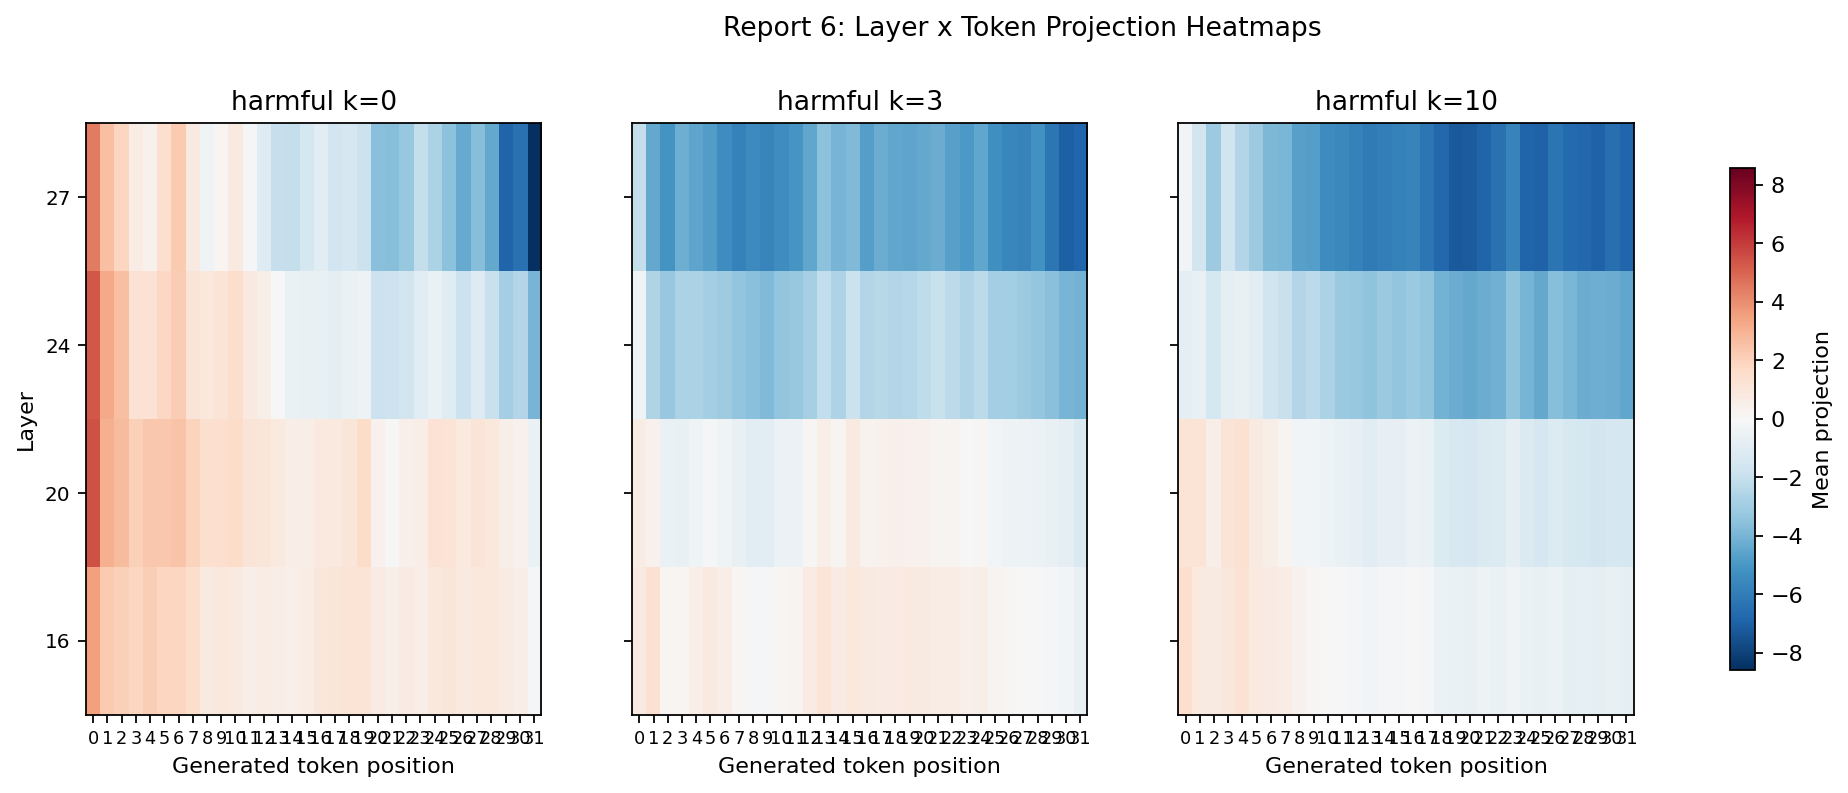
\includegraphics[width=0.95\linewidth]{figures/report6_heatmap_baseline_vs_prefill.png}
\caption{Mean refusal-direction projection by layer (rows) $\times$ generated
token position (columns) under harmful $k=0$, $k=3$, and $k=10$. Red is
positive (refusal-aligned), blue is negative (anti-refusal-aligned).
\textbf{Conclusion to draw:} under attack, layers 24 and 27 turn strongly
blue across most generated positions, while layers 16 and 20 shift only
mildly. The internal change is concentrated in late layers, consistent with
H2.}
\label{fig:heatmap}
\end{figure}

\begin{figure}[h]
\centering
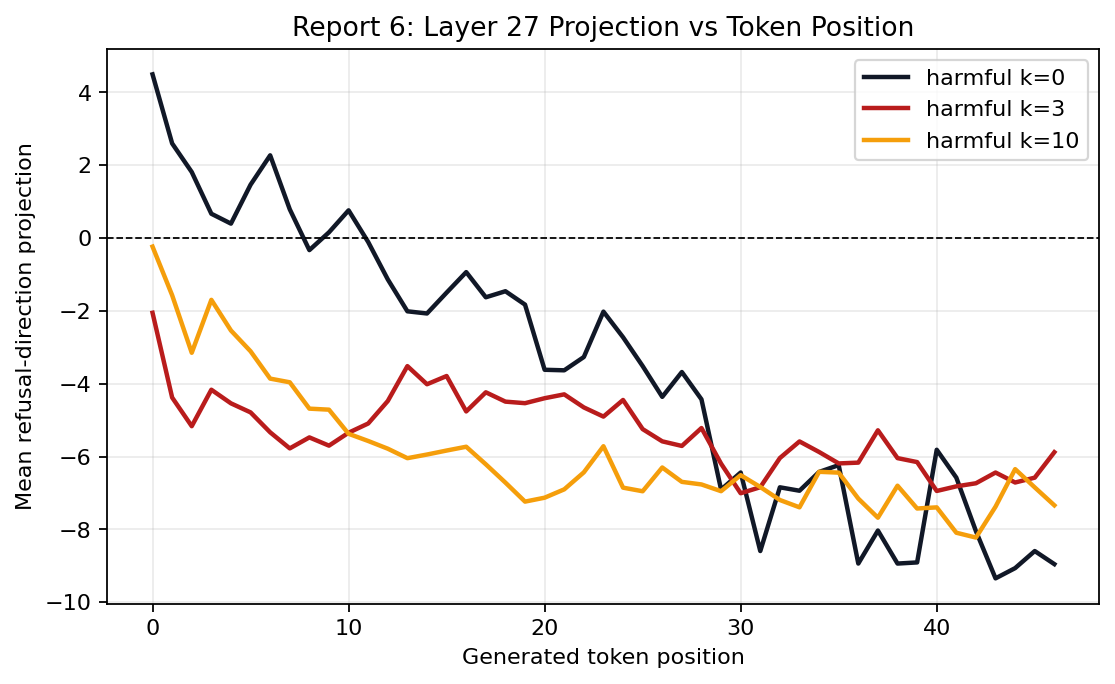
\includegraphics[width=0.49\linewidth]{figures/report6_projection_vs_token_layer27.png}
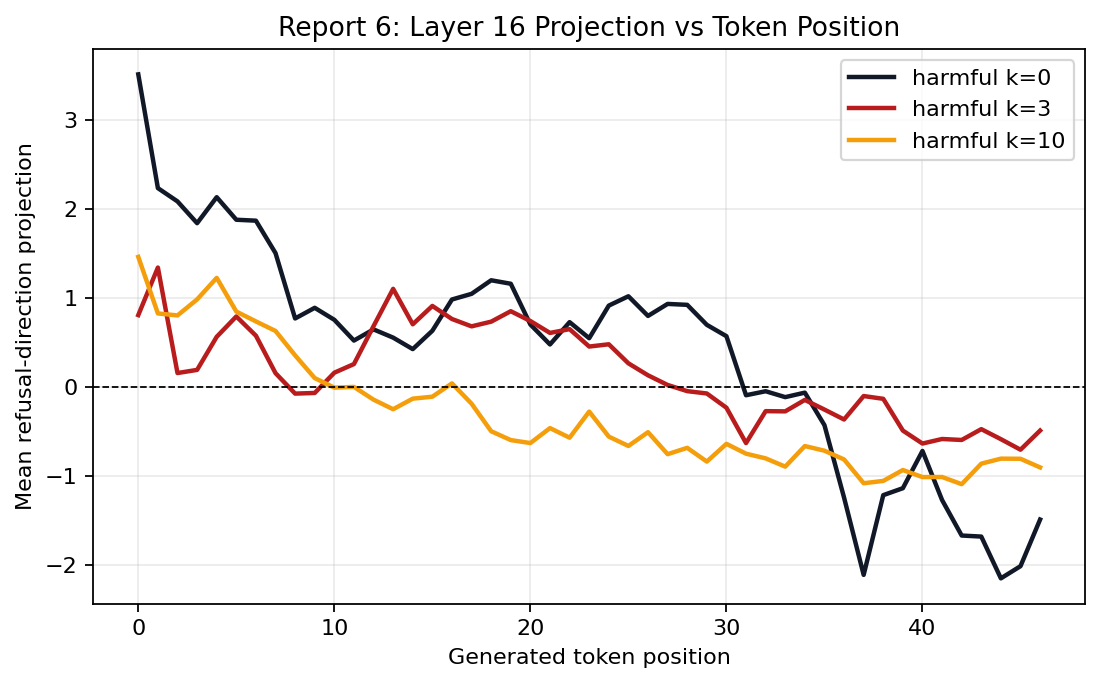
\includegraphics[width=0.49\linewidth]{figures/report6_projection_vs_token_layer16.png}
\caption{Mean refusal-direction projection vs.\ generated token position at
the late layer (left, layer 27) and at the comparison layer (right, layer
16) for harmful $k=0$, $k=3$, $k=10$. \textbf{Conclusion to draw:} at
layer~27, attacked traces are strongly negative across nearly all generated
positions and stay separated from $k=0$ for the early portion of the
response; at layer~16, all three curves stay close to zero and overlap heavily.
The attack-driven shift is much larger at the late layer than at the
comparison layer, consistent with H2.}
\label{fig:lines}
\end{figure}

The condition-level association predicted by H3 also holds in the same
direction. Refusal rate decreases (0.92 $\rightarrow$ 0.32) as the layer-27
mean projection becomes more negative ($-0.376 \rightarrow -5.285$). H3 is
therefore directionally supported at the condition level. A prompt-level
test (within $k=3$, do the 8 refusing prompts have less-negative late-layer
projection than the 17 complying prompts?) is not run in this report and is
listed as a Report~7 priority in Section~\ref{sec:conclusions}.

\section{Patching Results}
\label{sec:patching}

Table~\ref{tab:patching} summarizes the targeted patching grid under the
$k=3$ attack. The 10-prompt patching subset has a baseline refusal rate of
0.50 (5/10), so cells of interest are those that move the patched refusal
rate above 0.50.

\begin{table}[h]
\centering
\small
\caption{Targeted patching results under harmful $k=3$, on the same 10
prompts in every cell. Baseline refusal rate on the subset = 0.50 (5/10).
Source position is the last input/prefill token (\texttt{source\_pos}
$=-1$) of the same $k=3$ forward pass. Mean source projection is the mean
projection of that source activation onto the layer-specific
refusal-direction vector. \textbf{Conclusion to draw:} no cell restores
refusal; three cells slightly reduce it (one record flipped from refusal
to compliance in each). Across all 90 patching records: 0 restored,
3 lost, 87 no change. The layer-27 source projection is itself negative
($-0.458$) under $k=3$, so injecting that activation into early target
positions cannot be expected to restore refusal; the layer-24 source is
positive but still produces no restoration. Within this intervention
setting only, both H4 and H5 are not supported.}
\label{tab:patching}
\begin{tabular}{lrrrrrrr}
\toprule
Layer & Source proj.\ (mean) & \multicolumn{3}{c}{Patched refusal rate} & Restored & Lost & No change \\
\cmidrule(lr){3-5}
      &                  & $\text{tt}=1$ & $\text{tt}=3$ & $\text{tt}=5$ &          &      &           \\
\midrule
16 & $+0.543$ & 0.50 & 0.50 & 0.50 & 0 & 0 & 30 \\
24 & $+0.948$ & 0.40 & 0.40 & 0.50 & 0 & 2 & 28 \\
27 & $-0.458$ & 0.40 & 0.50 & 0.50 & 0 & 1 & 29 \\
\midrule
All cells &  &      &      &      & 0 & 3 & 87 \\
\bottomrule
\end{tabular}
\end{table}

\begin{figure}[!t]
\centering
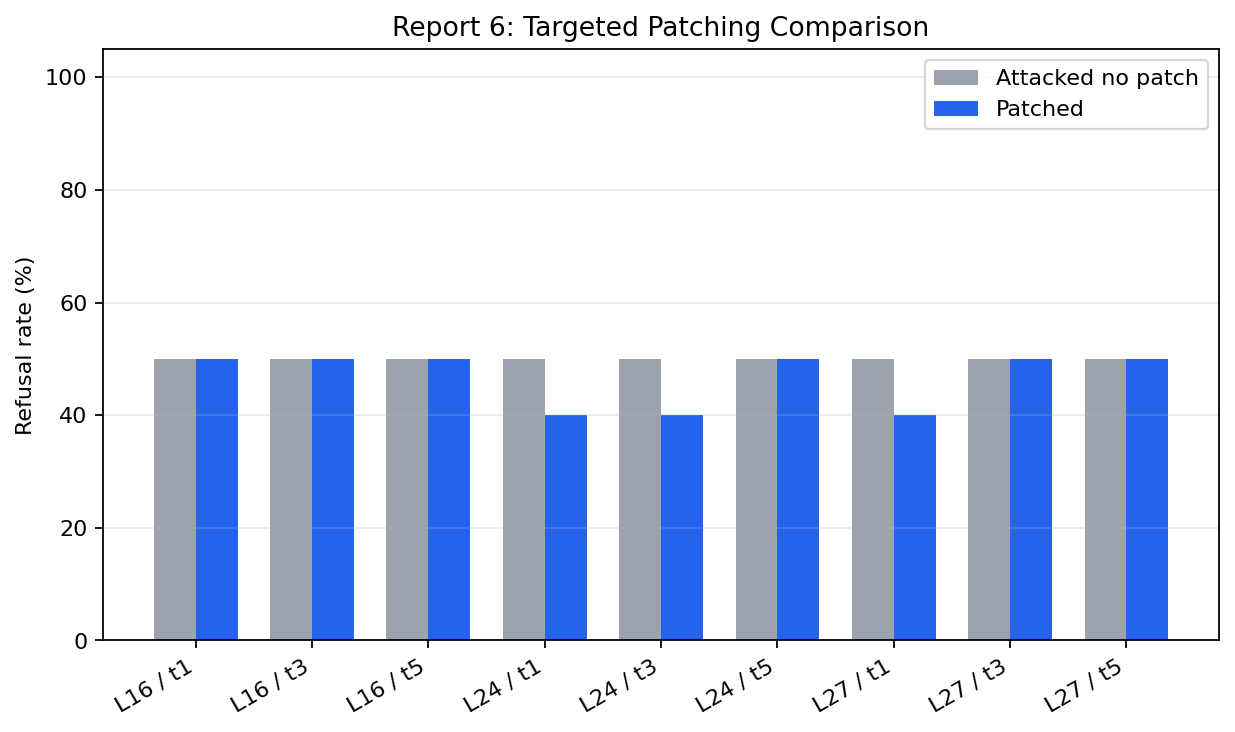
\includegraphics[width=0.7\linewidth]{figures/report6_patching_comparison.png}
\caption{Attacked-no-patch vs.\ patched refusal rate on the 10-prompt
subset for each (layer, target position) cell. \textbf{Conclusion to draw:}
no cell increases refusal above the 50\% attacked baseline. Three cells
(layer~24 / tt$=$1, layer~24 / tt$=$3, layer~27 / tt$=$1) drop from 50\%
to 40\% (one prompt flips from refusal to compliance in each). All other
cells are flat.}
\label{fig:patching}
\end{figure}

The patching block is a useful negative result for this specific
intervention setting. It does not show that refusal-direction interventions
cannot restore refusal in general, because the source state used here
(\texttt{source\_pos} $= -1$ from the same $k=3$ forward pass) may already
reflect the attacked context. At layer~27, the mean source projection is
$-0.458$, which is direct numerical evidence that the source is itself
inverted: the intervention is replacing an attacked state with another
attacked state at the same position. At layer~24, the source projection is
positive ($+0.948$), but this intervention still produced no restoration
in any cell. This suggests that source positivity alone is not sufficient
under the current same-condition patching design; testing whether a clean
$k=0$ source activation would behave differently is left to Report~7.

\FloatBarrier
\section{Updated Hypothesis Status}
\label{sec:hypstatus}

Table~\ref{tab:hyp} summarizes the hypothesis status; ``Status'' refers
strictly to the evidence collected in this report.

\begin{table}[!ht]
\centering
\small
\caption{Hypothesis status after Report~6 evidence.}
\label{tab:hyp}
\begin{tabular}{p{0.05\linewidth} p{0.18\linewidth} p{0.34\linewidth} p{0.30\linewidth}}
\toprule
H & Status & Evidence in this report & Next step \\
\midrule
H1 & Supported & Refusal drops 0.92 $\rightarrow$ 0.32 at $k=3$ on $n=25$
   harmful prompts; benign control 0.00. & Larger AdvBench sample in R7. \\
H2 & Supported & $|\Delta|$ from $k=0$ to $k=3$ grows monotonically with
   layer depth across $\{16,20,24,27\}$ ($1.10, 1.99, 3.78, 4.91$). &
   Add intermediate layers; check held-out direction. \\
H3 & Directionally consistent at the condition level; not yet tested at the
   prompt level & Refusal rate moves with layer-27 mean projection across
   $k\in\{0,3\}$. & Within-$k=3$ prompt-level association. \\
H4 & Not supported under current intervention design & 0/90 restored across
   the 9 cells; layer-27 source itself inverted ($-0.458$). & Use $k=0$
   source activations; revisit. \\
H5 & Not supported under current intervention design;
   not fairly evaluable & No layer beats 50\% attacked baseline; weakest
   evidence comes from the layer with negative source. & Re-test after
   fixing source. \\
\bottomrule
\end{tabular}
\end{table}
\FloatBarrier

\section{Conclusions and Threats to Validity}
\label{sec:conclusions}

\subsection{Main conclusions}

Report~6 reproduces the behavioral prefilling attack effect and the
late-layer negative shift in the refusal-direction projection in a single
focused design on Llama-3.1-8B-Instruct. The behavioral drop and the
late-layer shift co-occur at the condition level, and both are much weaker
at the comparison layer~16 than at layers 24 and 27. Within the specific
patching design used here---same-condition self-patching of the
last-input-token activation into early generated positions---no cell
restores refusal, and three cells slightly reduce it. The layer-27 source
projection under $k=3$ is itself negative, which mechanistically explains
why this intervention setting is not a fair test of the broader
restoration hypothesis. The contribution of Report~6 versus Report~3 is
therefore narrower and more diagnostic than ``confirms the mechanism'':
it replicates the late-layer pattern with a redesigned narrower pipeline,
quantifies the layer-by-layer shift on a common generated-token averaging
window, and adds a 9-cell intervention grid whose null result is
interpretable because the source projection is recorded per cell.

\subsection{Priorities for Report 7}

Report~7 should improve the intervention design before drawing stronger
causal conclusions:

\begin{enumerate}
\item Use $k=0$ baseline activations from the same prompt as the patching
  source, rather than activations from the attacked $k=3$ forward pass.
  This is the standard activation-patching design and the single highest-
  priority change.
\item Add a prompt-level association test inside $k=3$: do the 8 refusing
  prompts have less-negative layer-24 / 27 mean projection than the 17
  complying prompts? This is a no-cost addition from existing trace data
  and would directly address the H3 caveat.
\item Concentrate the patching grid on layers 24 and 27 only, but expand
  target positions to include position 0 and to span a wider early window.
  The refusal commitment in Llama-style chat models is often visible at the
  very first generated token.
\item Re-run harmful $k=10$ behavioral generation on a compatible GPU so
  the entire behavioral table is inside the Report~6 pipeline. The current
  $k=10$ row uses Report~3 exploratory data only.
\item Optionally, evaluate a held-out refusal direction (extracted from
  prompts disjoint from the traced subset) to address the direction-overfitting
  concern in Section~\ref{sec:threats}.
\end{enumerate}

\subsection{Threats to validity}
\label{sec:threats}

\paragraph{Internal validity.}
The phrase-list refusal classifier inspects only the first $\approx$200
characters of the model's response and has known failure modes (e.g.,
``I cannot stress enough\ldots'' as a false positive); a small number of
borderline outputs may be mislabeled and the refusal counts in
Table~\ref{tab:behavior} are an approximation, not a content judgment.
The patching source is taken from the same $k=3$ attacked forward pass at
\texttt{source\_pos} $= -1$, which is not a clean refusal-aligned state---at
layer~27 it is in fact already inverted (mean source projection $-0.458$).
The null result in Section~\ref{sec:patching} therefore reflects this
intervention design and does not provide evidence that
refusal-direction interventions cannot restore refusal in general. The
patching subset is 10 prompts; small per-cell effects (one or two
prompts flipping) are within sampling noise and are not interpreted
substantively. The refusal direction was extracted from 50 harmful + 50
benign prompts that include the 25 traced prompts, so projection magnitudes
may be modestly inflated relative to a held-out direction. Trace summaries
average over generated-token positions; short refusals and long compliant
continuations contribute different numbers of records to the same mean,
and we report the same generated-token averaging window in every row of
Table~\ref{tab:tracing} but do not separate early- vs.\ late-position
windows in this report.

\paragraph{External validity.}
All results come from a single model (Llama-3.1-8B-Instruct), one attack
family (prefilling with fixed prefix length $k$), $n=25$ harmful prompts
from one benchmark (AdvBench), and greedy decoding. Late-layer specificity
patterns may differ for other safety-aligned model families, for suffix-style
attacks~\cite{zou2023advbench}, or under sampled decoding. The patching
subset is a further restriction to 10 prompts.

\paragraph{Construct validity.}
The refusal-direction projection is a proxy for one dimension of refusal-related
internal state, not a complete representation of safety. A
sufficiently-aligned model could, in principle, refuse via mechanisms that
the difference-in-means direction does not capture, such as specific safety
neurons~\cite{chen2025safetyneurons} or attention heads~\cite{zhou2025safetyheads}.
Projection magnitudes are layer-specific (each layer has its own
direction vector), so absolute values are not comparable across layers and
should be interpreted as within-layer changes. The behavioral refusal label is
a proxy for ``did the model refuse,'' not for whether the response is
harmful, and is not equivalent to a guard-model-style harmfulness assessment.

{\small
\bibliographystyle{abbrv}
\bibliography{references}
}

\end{document}
